\documentclass[a4j]{jarticle}

\usepackage{amsmath}	% required for `\align' (yatex added)
\usepackage{graphicx}[dvipdfmx]	% required for `\includegraphics' (yatex added)
\begin{document}

\section{試してみる}
テスト数式
\begin{align}
 120+200=320\label{150320_12Nov19}
\end{align}
式\ref{150320_12Nov19}は,,,

\section{何をやっているか}
式を書いてみる.例えば
\begin{align}
 20+30+40=90\label{151751_12Nov19}
\end{align}
みたいな.yatexのrefは,わざわざ自分でlabelをつけなくても,C\_c sのsection型補完でrefと打つと,それっぽいところをいくつかピックアップしてくれるという素晴らしい機能を持っている.https://www.yatex.org/qanda.htmlに,


\begin{quotation}
 %\textbackslashでバックスラッシュを出力することができる.\\ではないので注意. 
 ・RefTeXは使えますか?
	
	使っている人はいるみたいですから使えるんじゃないでしょうか。でも
	ですね、野鳥の \textbackslash ref 補完があれば、RefTeXなんぞ要らないと思います
	よ。これからは \textbackslash label\{\}はいちいち自分では作らずにいきなり[prefix]
	s で \textbackslash ref を打ち込みましょう。勝手にラベルを打てそうなところを探
	して勝手にラベルを打ってその名前を \textbackslash refに入れてくれます。 \textbackslash ref補完
	は  \textbackslash label\{\} と  \textbackslash ref\{\} 両方同時に補完入力します。
\end{quotation}	
と書いてある.

実際にセクション型補完で\textbackslash ref と打ってみると,
\begin{figure}[htb]
 \centering
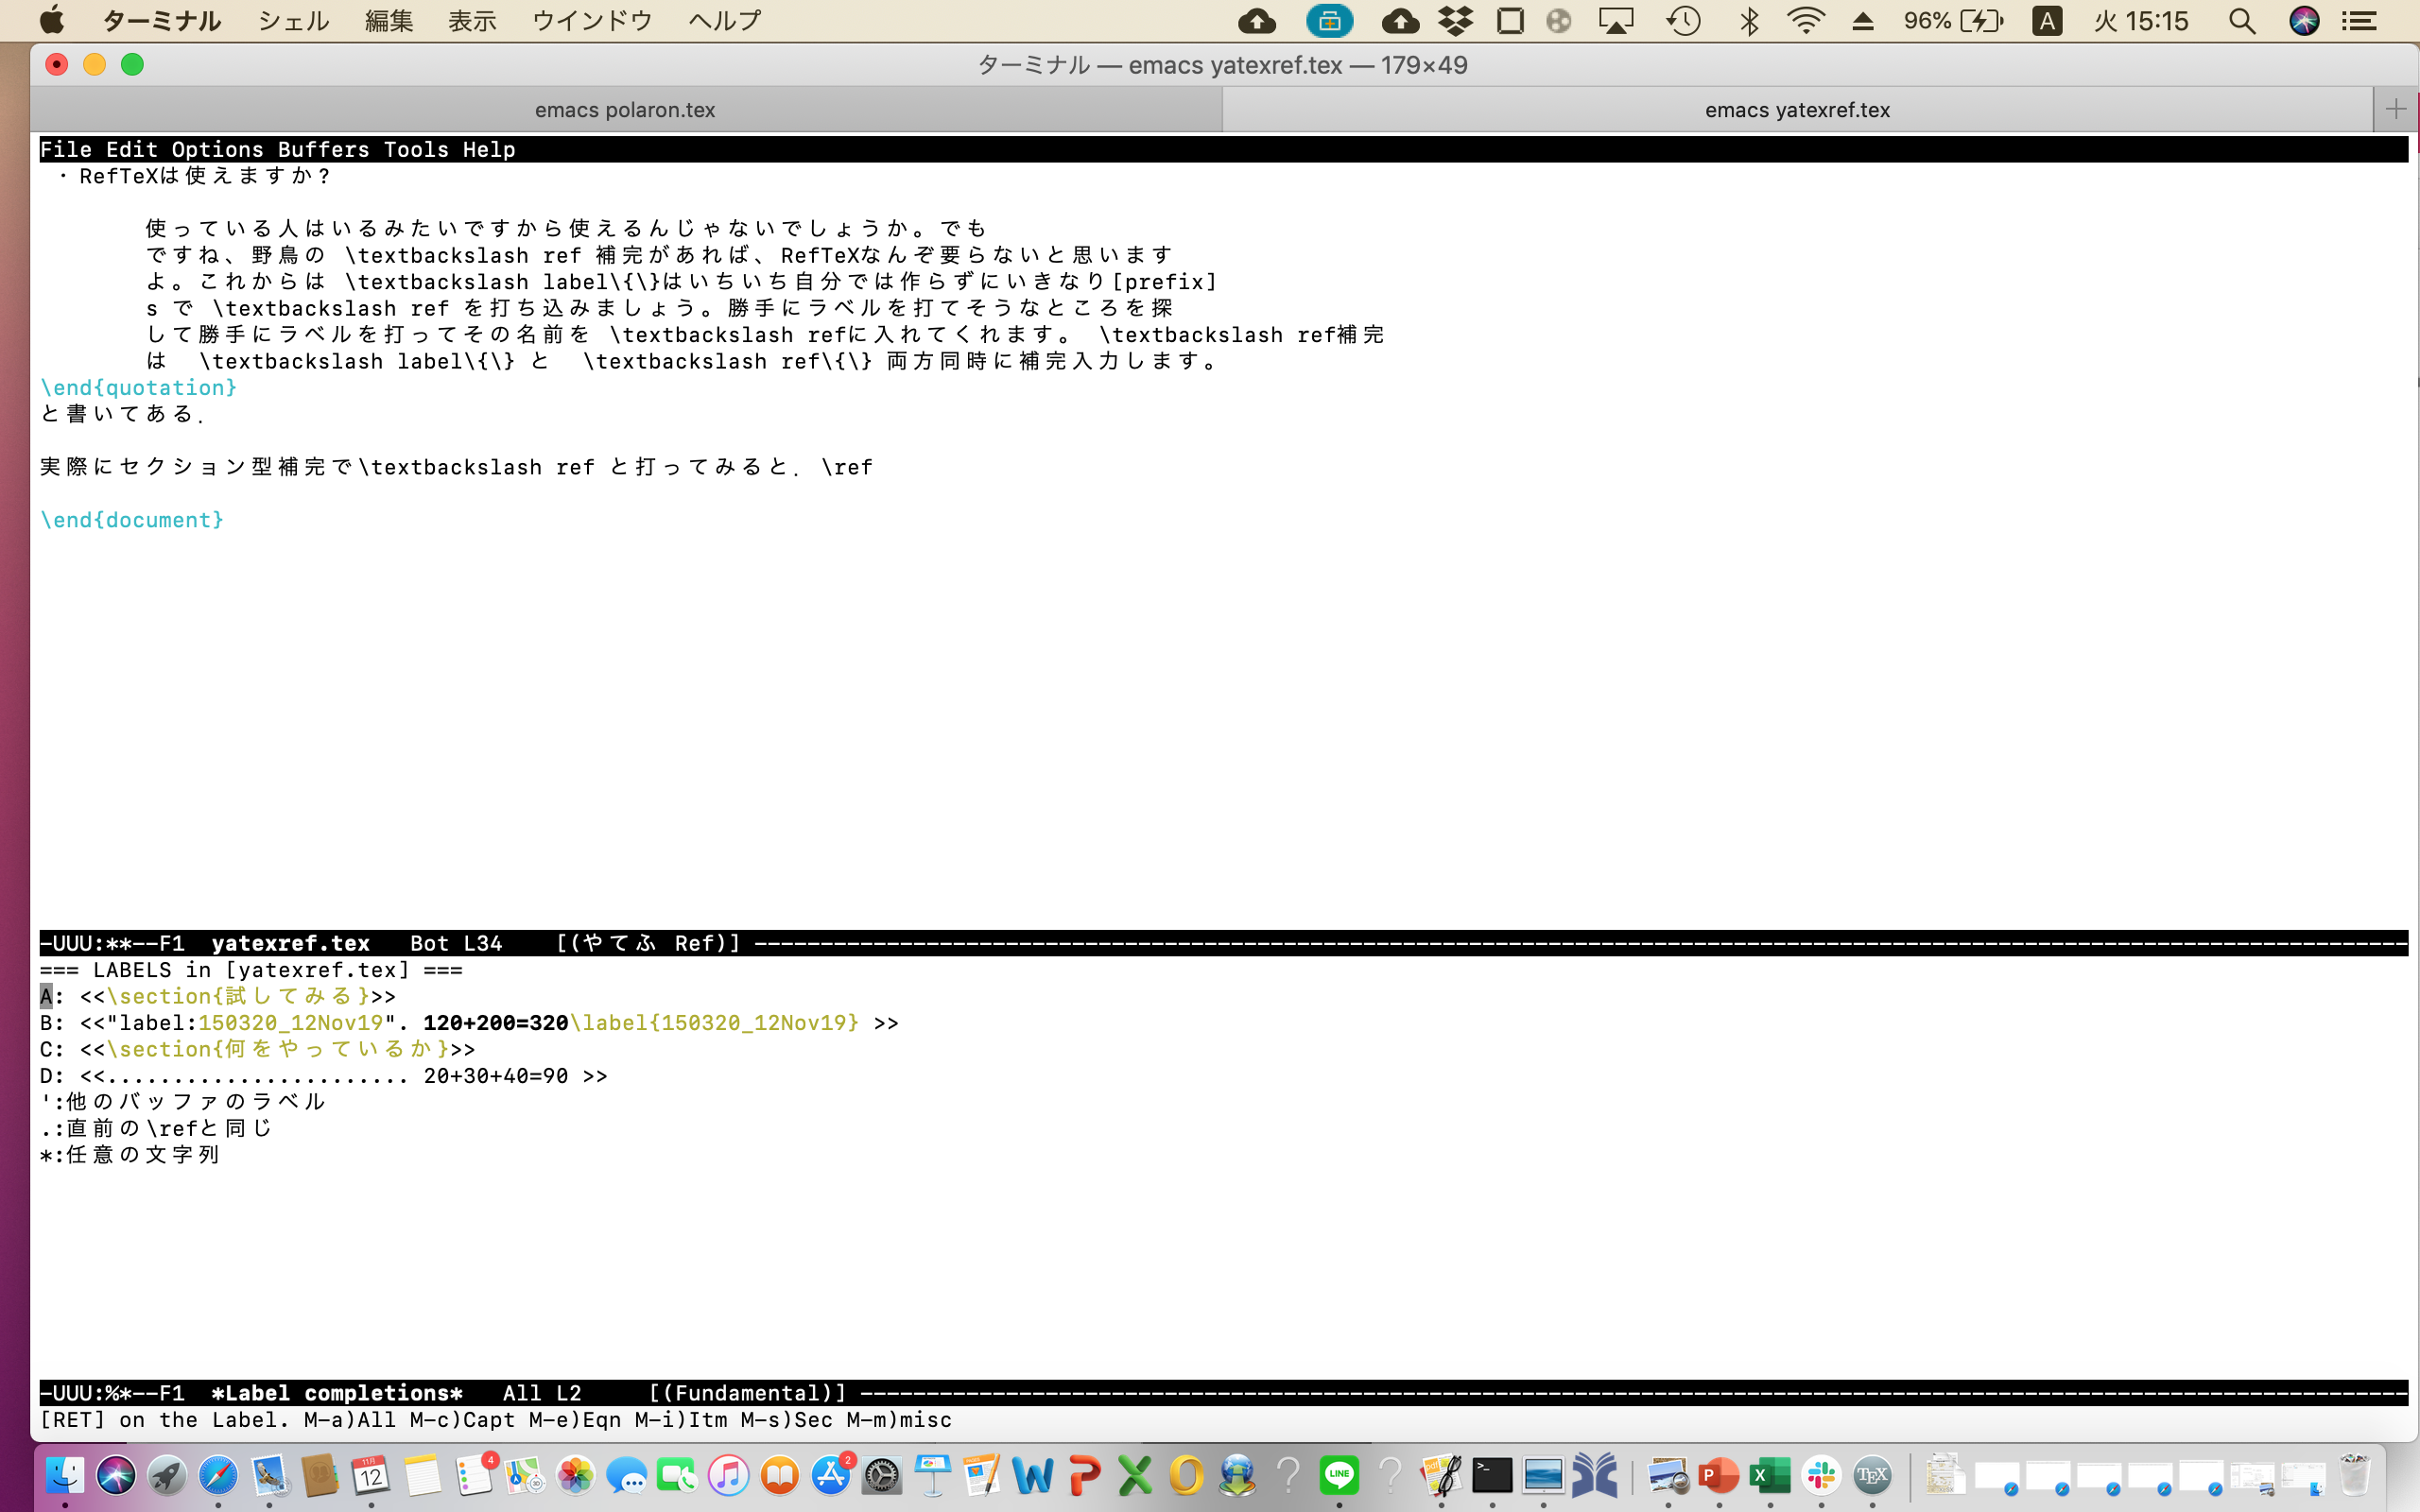
\includegraphics[bb=0 0 2560 1600,width=5cm]{スクリーンショット 2019-11-12 15.15.29.png}
\end{figure}
となって,適当にRETで選択することができる.ちなみにeqrefでも可能であるのが嬉しい.RETを押すと,
\begin{figure}[htb]
 \centering
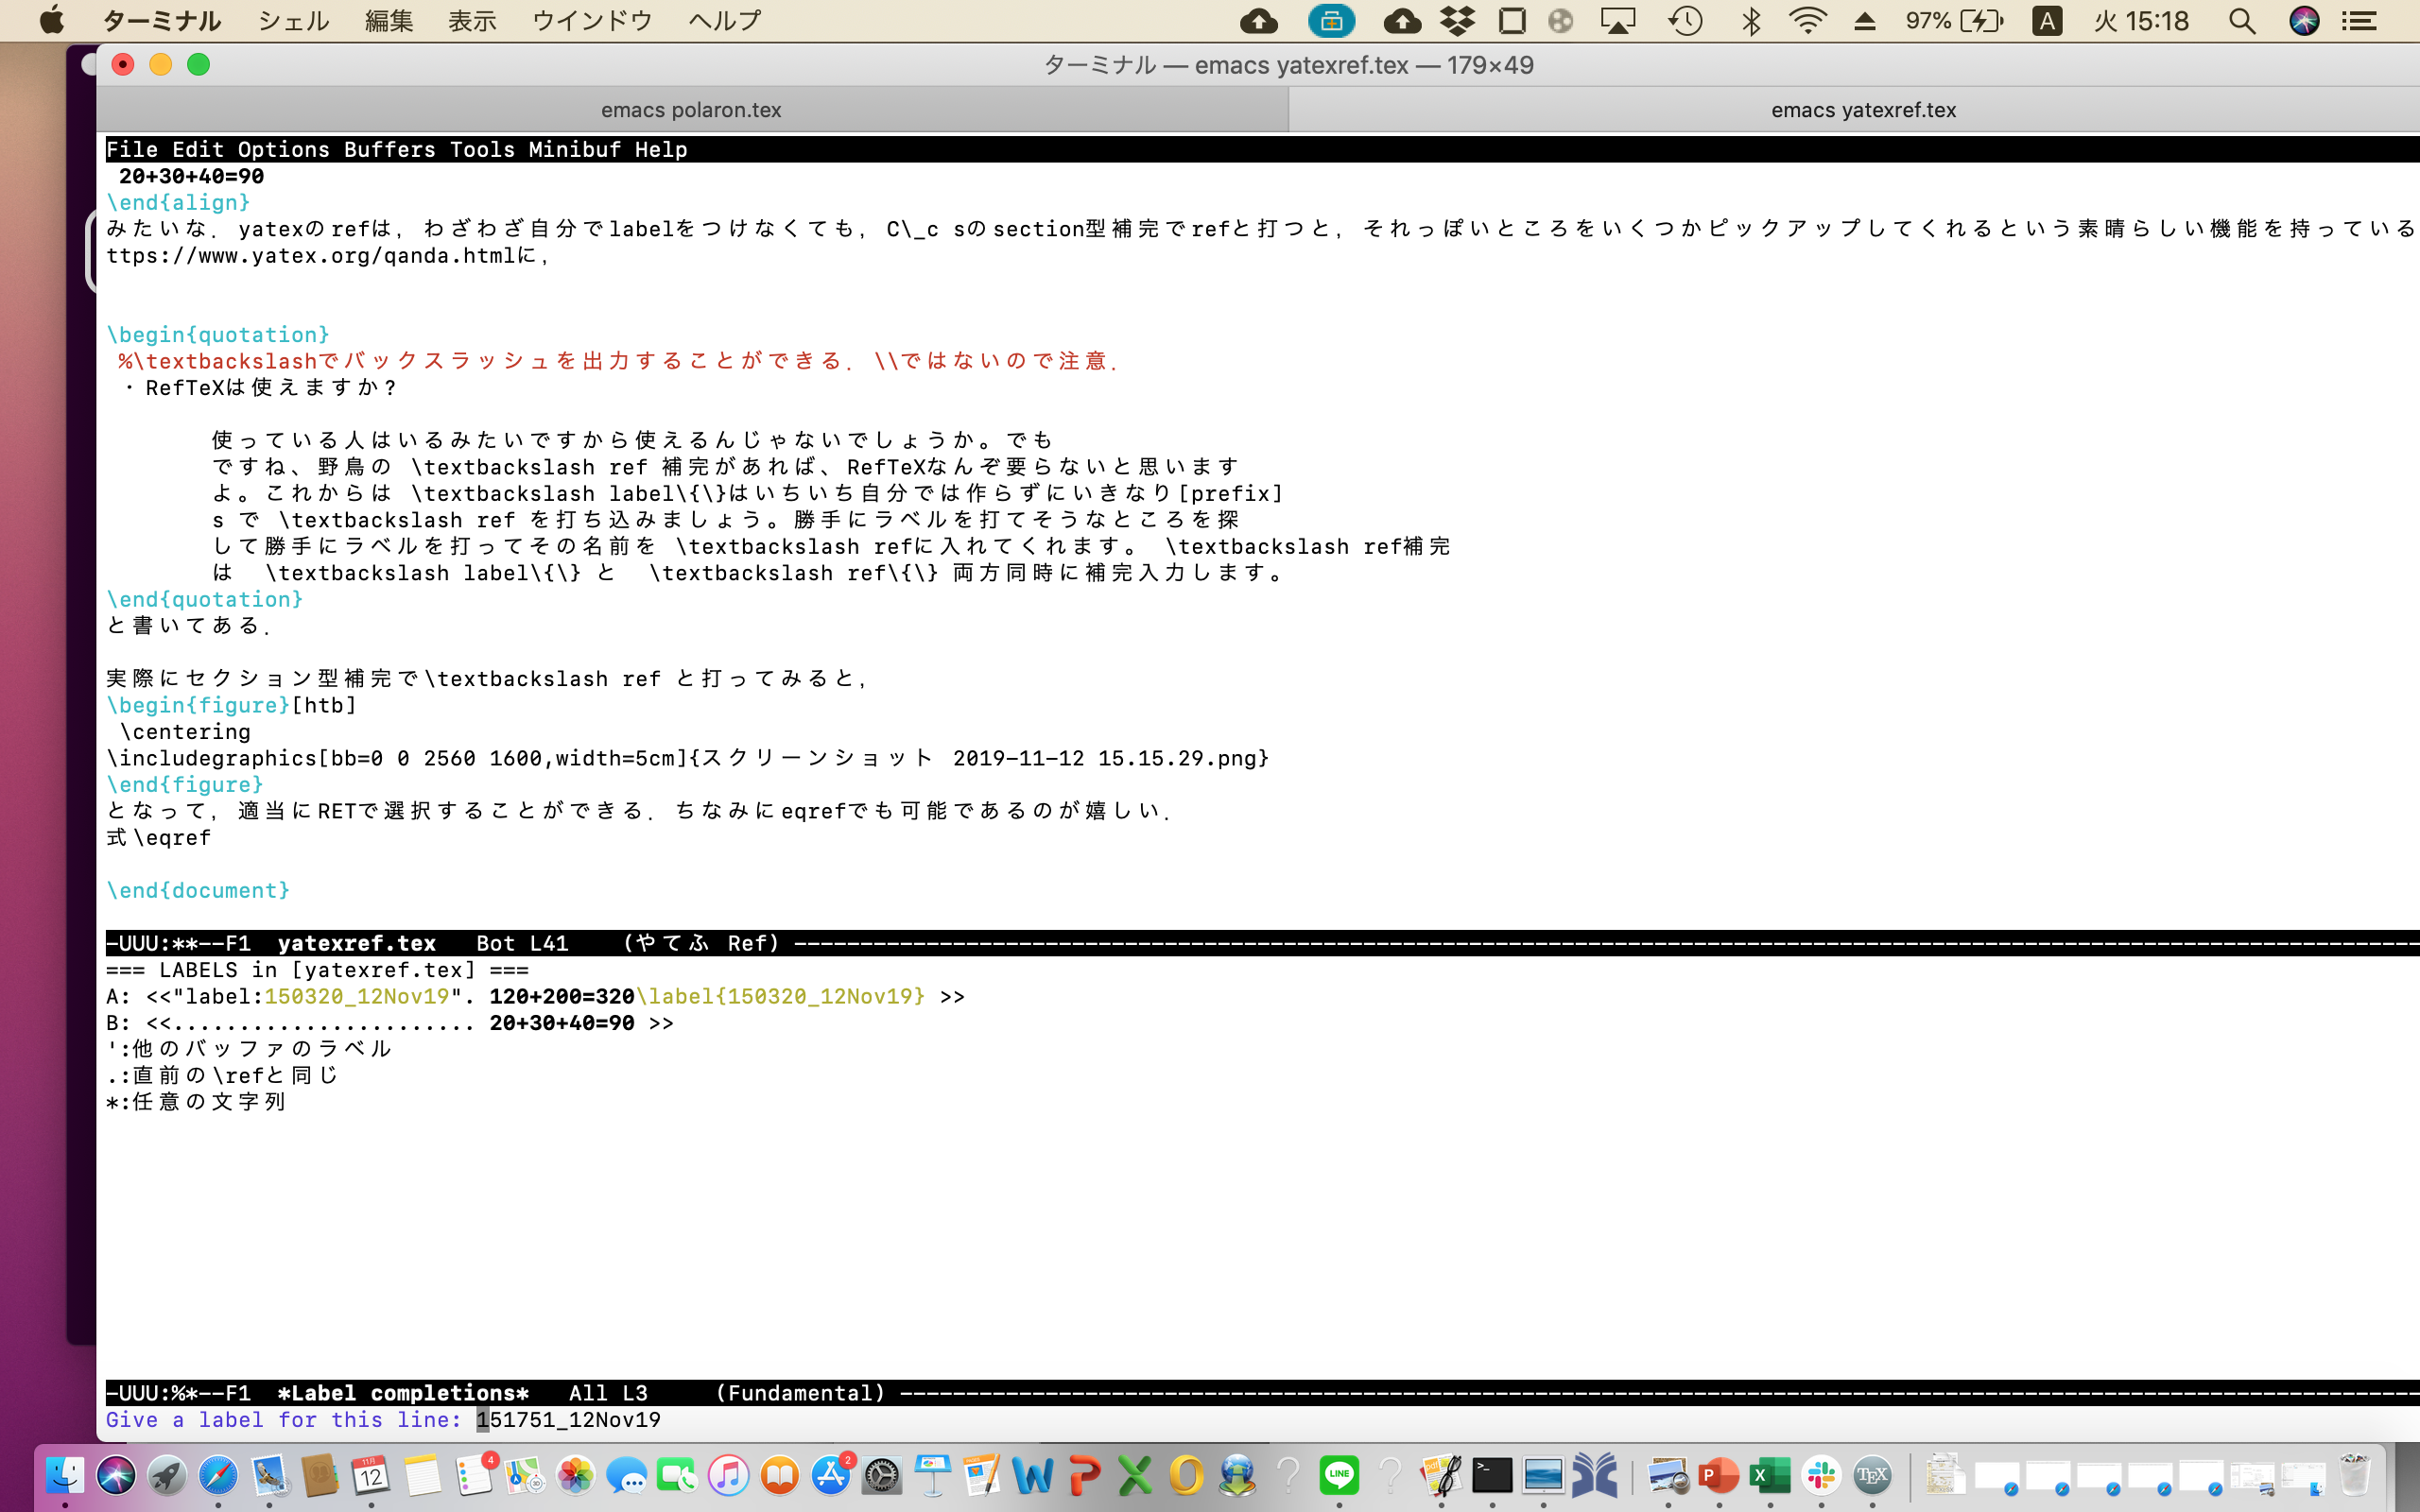
\includegraphics[bb=0 0 2560 1600,width=5cm]{スクリーンショット 2019-11-12 15.18.05.png}
\end{figure}
となって,labelの名前も自分で打つことができる.デフォルトは時間になっている.


式\eqref{151751_12Nov19}的な感じ.

\end{document}